\documentclass{standalone}
\usepackage{tikz}
\usetikzlibrary{patterns, positioning}


\begin{document}
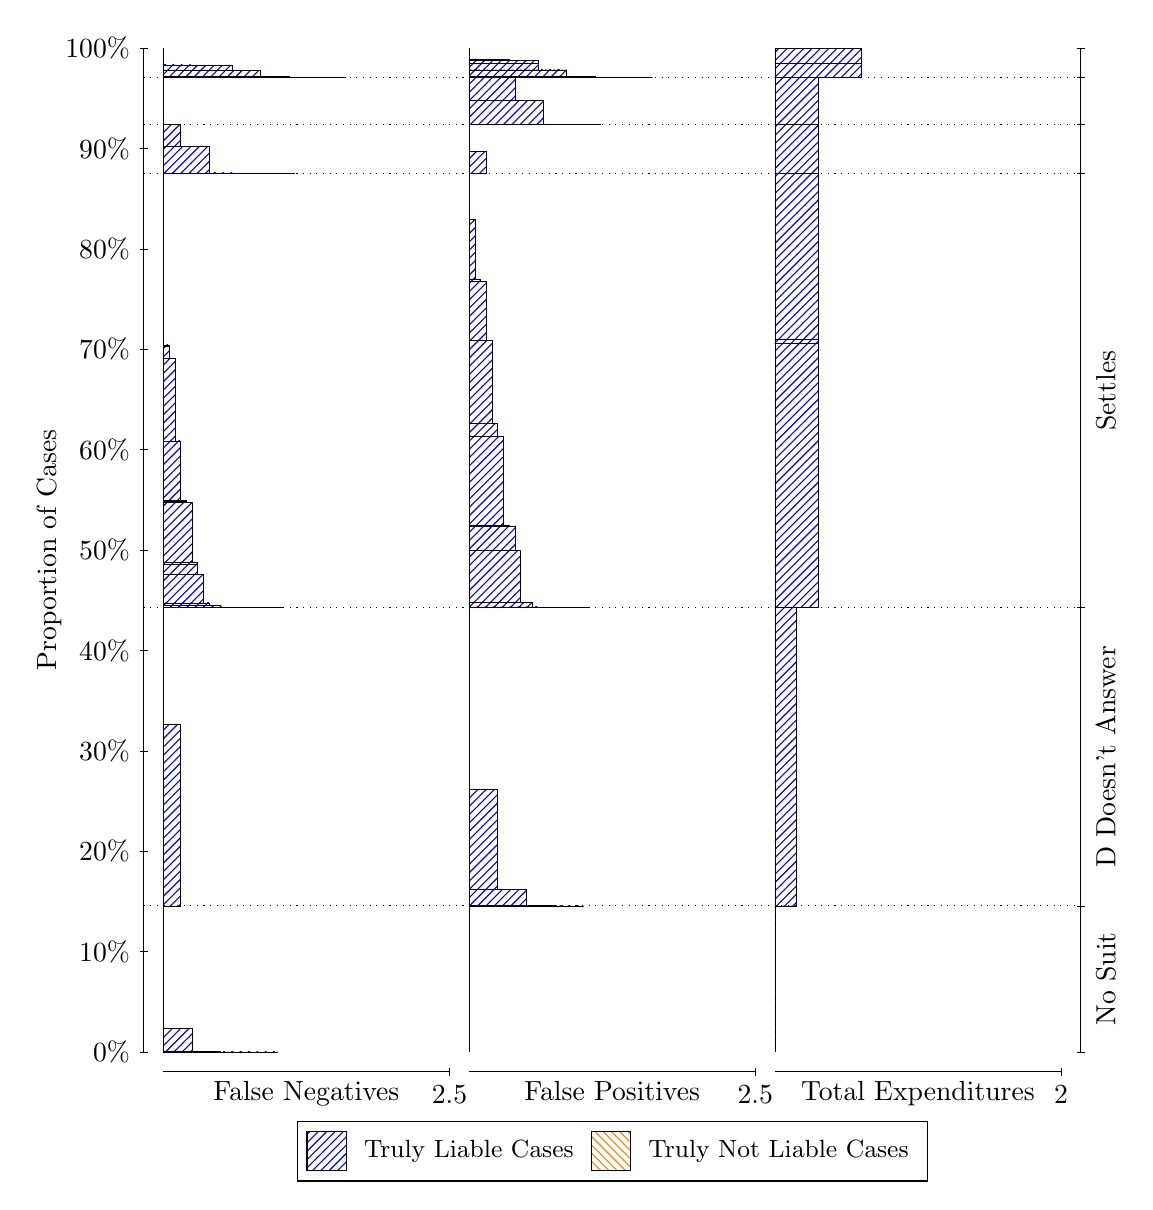
\begin{tikzpicture}
\draw[black, very thin] (1.5,1.75) -- (1.5,14.5);
\node[rotate=90, text=black, anchor=center] at (0.3, 8.125) {Proportion of Cases};
\draw[black, very thin] (1.45,1.75) -- (1.55,1.75);
\node[text=black, anchor=east] at (1.45, 1.75) {0\%};
\draw[black, very thin] (1.45,3.025) -- (1.55,3.025);
\node[text=black, anchor=east] at (1.45, 3.025) {10\%};
\draw[black, very thin] (1.45,4.3) -- (1.55,4.3);
\node[text=black, anchor=east] at (1.45, 4.3) {20\%};
\draw[black, very thin] (1.45,5.575) -- (1.55,5.575);
\node[text=black, anchor=east] at (1.45, 5.575) {30\%};
\draw[black, very thin] (1.45,6.85) -- (1.55,6.85);
\node[text=black, anchor=east] at (1.45, 6.85) {40\%};
\draw[black, very thin] (1.45,8.125) -- (1.55,8.125);
\node[text=black, anchor=east] at (1.45, 8.125) {50\%};
\draw[black, very thin] (1.45,9.4) -- (1.55,9.4);
\node[text=black, anchor=east] at (1.45, 9.4) {60\%};
\draw[black, very thin] (1.45,10.675) -- (1.55,10.675);
\node[text=black, anchor=east] at (1.45, 10.675) {70\%};
\draw[black, very thin] (1.45,11.95) -- (1.55,11.95);
\node[text=black, anchor=east] at (1.45, 11.95) {80\%};
\draw[black, very thin] (1.45,13.225) -- (1.55,13.225);
\node[text=black, anchor=east] at (1.45, 13.225) {90\%};
\draw[black, very thin] (1.45,14.5) -- (1.55,14.5);
\node[text=black, anchor=east] at (1.45, 14.5) {100\%};

\draw[black, very thin] (13.4,1.75) -- (13.4,14.5);
\draw[black, very thin] (13.35,1.75) -- (13.45,1.75);
\node[anchor=west] at (13.35, 1.75) {};
\draw[black, very thin] (13.35,3.6057) -- (13.45,3.6057);
\node[anchor=west] at (13.35, 3.6057) {};
\draw[black, very thin] (13.35,7.3916) -- (13.45,7.3916);
\node[anchor=west] at (13.35, 7.3916) {};
\draw[black, very thin] (13.35,12.905) -- (13.45,12.905);
\node[anchor=west] at (13.35, 12.905) {};
\draw[black, very thin] (13.35,13.526) -- (13.45,13.526);
\node[anchor=west] at (13.35, 13.526) {};
\draw[black, very thin] (13.35,14.13) -- (13.45,14.13);
\node[anchor=west] at (13.35, 14.13) {};
\draw[black, very thin] (13.35,14.5) -- (13.45,14.5);
\node[anchor=west] at (13.35, 14.5) {};

\draw[black, very thin, pattern color=blue, pattern=north east lines] (1.75,1.75) rectangle (3.2033,1.75);
\draw[black, very thin, pattern color=blue, pattern=north east lines] (1.75,1.75) rectangle (2.84,1.75);
\draw[black, very thin, pattern color=blue, pattern=north east lines] (1.75,1.75) rectangle (2.4767,1.7526);
\draw[black, very thin, pattern color=blue, pattern=north east lines] (1.75,1.7526) rectangle (2.1133,2.0538);
\draw[black, very thin, pattern color=orange, pattern=north west lines] (1.75,2.0538) rectangle (1.75,2.0538);
\draw[black, very thin, pattern color=blue, pattern=north east lines] (1.75,2.0538) rectangle (1.75,3.6057);
\draw[black, very thin, pattern color=blue, pattern=north east lines] (1.75,3.6057) rectangle (1.968,5.9132);
\draw[black, very thin, pattern color=orange, pattern=north west lines] (1.75,5.9132) rectangle (1.75,5.9132);
\draw[black, very thin, pattern color=blue, pattern=north east lines] (1.75,5.9132) rectangle (1.75,7.3916);
\draw[black, very thin, pattern color=blue, pattern=north east lines] (1.75,7.3916) rectangle (3.276,7.3916);
\draw[black, very thin, pattern color=blue, pattern=north east lines] (1.75,7.3916) rectangle (3.1307,7.3916);
\draw[black, very thin, pattern color=blue, pattern=north east lines] (1.75,7.3916) rectangle (2.9853,7.3916);
\draw[black, very thin, pattern color=blue, pattern=north east lines] (1.75,7.3916) rectangle (2.9127,7.3916);
\draw[black, very thin, pattern color=blue, pattern=north east lines] (1.75,7.3916) rectangle (2.84,7.3916);
\draw[black, very thin, pattern color=blue, pattern=north east lines] (1.75,7.3916) rectangle (2.7673,7.3916);
\draw[black, very thin, pattern color=blue, pattern=north east lines] (1.75,7.3916) rectangle (2.6947,7.3916);
\draw[black, very thin, pattern color=blue, pattern=north east lines] (1.75,7.3916) rectangle (2.622,7.4002);
\draw[black, very thin, pattern color=blue, pattern=north east lines] (1.75,7.4002) rectangle (2.5493,7.4013);
\draw[black, very thin, pattern color=blue, pattern=north east lines] (1.75,7.4013) rectangle (2.4767,7.4202);
\draw[black, very thin, pattern color=blue, pattern=north east lines] (1.75,7.4202) rectangle (2.404,7.4202);
\draw[black, very thin, pattern color=blue, pattern=north east lines] (1.75,7.4202) rectangle (2.404,7.4209);
\draw[black, very thin, pattern color=blue, pattern=north east lines] (1.75,7.4209) rectangle (2.3313,7.4539);
\draw[black, very thin, pattern color=blue, pattern=north east lines] (1.75,7.4539) rectangle (2.2587,7.82);
\draw[black, very thin, pattern color=blue, pattern=north east lines] (1.75,7.82) rectangle (2.186,7.9375);
\draw[black, very thin, pattern color=blue, pattern=north east lines] (1.75,7.9375) rectangle (2.186,7.966);
\draw[black, very thin, pattern color=blue, pattern=north east lines] (1.75,7.966) rectangle (2.1133,8.7295);
\draw[black, very thin, pattern color=blue, pattern=north east lines] (1.75,8.7295) rectangle (2.0407,8.7448);
\draw[black, very thin, pattern color=blue, pattern=north east lines] (1.75,8.7448) rectangle (2.0407,8.7572);
\draw[black, very thin, pattern color=blue, pattern=north east lines] (1.75,8.7572) rectangle (1.968,9.5111);
\draw[black, very thin, pattern color=blue, pattern=north east lines] (1.75,9.5111) rectangle (1.8953,10.561);
\draw[black, very thin, pattern color=blue, pattern=north east lines] (1.75,10.561) rectangle (1.8227,10.708);
\draw[black, very thin, pattern color=blue, pattern=north east lines] (1.75,10.708) rectangle (1.8227,10.731);
\draw[black, very thin, pattern color=orange, pattern=north west lines] (1.75,10.731) rectangle (1.75,10.731);
\draw[black, very thin, pattern color=blue, pattern=north east lines] (1.75,10.731) rectangle (1.75,12.905);
\draw[black, very thin, pattern color=blue, pattern=north east lines] (1.75,12.905) rectangle (3.4213,12.905);
\draw[black, very thin, pattern color=blue, pattern=north east lines] (1.75,12.905) rectangle (3.058,12.905);
\draw[black, very thin, pattern color=blue, pattern=north east lines] (1.75,12.905) rectangle (2.6947,12.913);
\draw[black, very thin, pattern color=blue, pattern=north east lines] (1.75,12.913) rectangle (2.3313,13.247);
\draw[black, very thin, pattern color=blue, pattern=north east lines] (1.75,13.247) rectangle (1.968,13.526);
\draw[black, very thin, pattern color=orange, pattern=north west lines] (1.75,13.526) rectangle (1.75,13.526);
\draw[black, very thin, pattern color=blue, pattern=north east lines] (1.75,13.526) rectangle (1.968,13.53);
\draw[black, very thin, pattern color=orange, pattern=north west lines] (1.75,13.53) rectangle (1.75,13.53);
\draw[black, very thin, pattern color=blue, pattern=north east lines] (1.75,13.53) rectangle (1.75,14.13);
\draw[black, very thin, pattern color=blue, pattern=north east lines] (1.75,14.13) rectangle (4.0753,14.13);
\draw[black, very thin, pattern color=blue, pattern=north east lines] (1.75,14.13) rectangle (3.712,14.13);
\draw[black, very thin, pattern color=blue, pattern=north east lines] (1.75,14.13) rectangle (3.3487,14.135);
\draw[black, very thin, pattern color=blue, pattern=north east lines] (1.75,14.135) rectangle (2.9853,14.212);
\draw[black, very thin, pattern color=blue, pattern=north east lines] (1.75,14.212) rectangle (2.84,14.212);
\draw[black, very thin, pattern color=blue, pattern=north east lines] (1.75,14.212) rectangle (2.622,14.275);
\draw[black, very thin, pattern color=blue, pattern=north east lines] (1.75,14.275) rectangle (2.4767,14.275);
\draw[black, very thin, pattern color=blue, pattern=north east lines] (1.75,14.275) rectangle (2.2587,14.276);
\draw[black, very thin, pattern color=blue, pattern=north east lines] (1.75,14.276) rectangle (2.1133,14.285);
\draw[black, very thin, pattern color=blue, pattern=north east lines] (1.75,14.285) rectangle (1.8953,14.285);
\draw[black, very thin, pattern color=orange, pattern=north west lines] (1.75,14.285) rectangle (1.75,14.285);
\draw[black, very thin, pattern color=blue, pattern=north east lines] (1.75,14.285) rectangle (1.75,14.5);
\draw[black, very thin, pattern color=orange, pattern=north west lines] (5.6333,1.75) rectangle (5.6333,1.75);
\draw[black, very thin, pattern color=blue, pattern=north east lines] (5.6333,1.75) rectangle (5.6333,3.6057);
\draw[black, very thin, pattern color=orange, pattern=north west lines] (5.6333,3.6057) rectangle (7.0867,3.6057);
\draw[black, very thin, pattern color=blue, pattern=north east lines] (5.6333,3.6057) rectangle (7.0867,3.6057);
\draw[black, very thin, pattern color=blue, pattern=north east lines] (5.6333,3.6057) rectangle (6.7233,3.6072);
\draw[black, very thin, pattern color=blue, pattern=north east lines] (5.6333,3.6072) rectangle (6.36,3.8109);
\draw[black, very thin, pattern color=blue, pattern=north east lines] (5.6333,3.8109) rectangle (5.9967,5.0842);
\draw[black, very thin, pattern color=blue, pattern=north east lines] (5.6333,5.0842) rectangle (5.6333,7.3916);
\draw[black, very thin, pattern color=orange, pattern=north west lines] (5.6333,7.3916) rectangle (7.1593,7.3916);
\draw[black, very thin, pattern color=blue, pattern=north east lines] (5.6333,7.3916) rectangle (7.1593,7.3916);
\draw[black, very thin, pattern color=orange, pattern=north west lines] (5.6333,7.3916) rectangle (6.8687,7.3916);
\draw[black, very thin, pattern color=blue, pattern=north east lines] (5.6333,7.3916) rectangle (6.8687,7.3916);
\draw[black, very thin, pattern color=blue, pattern=north east lines] (5.6333,7.3916) rectangle (6.796,7.3917);
\draw[black, very thin, pattern color=orange, pattern=north west lines] (5.6333,7.3917) rectangle (6.7233,7.3917);
\draw[black, very thin, pattern color=blue, pattern=north east lines] (5.6333,7.3917) rectangle (6.7233,7.3917);
\draw[black, very thin, pattern color=orange, pattern=north west lines] (5.6333,7.3917) rectangle (6.578,7.3917);
\draw[black, very thin, pattern color=blue, pattern=north east lines] (5.6333,7.3917) rectangle (6.578,7.4021);
\draw[black, very thin, pattern color=blue, pattern=north east lines] (5.6333,7.4021) rectangle (6.5053,7.4021);
\draw[black, very thin, pattern color=orange, pattern=north west lines] (5.6333,7.4021) rectangle (6.4327,7.4021);
\draw[black, very thin, pattern color=blue, pattern=north east lines] (5.6333,7.4021) rectangle (6.4327,7.455);
\draw[black, very thin, pattern color=blue, pattern=north east lines] (5.6333,7.455) rectangle (6.36,7.4565);
\draw[black, very thin, pattern color=orange, pattern=north west lines] (5.6333,7.4565) rectangle (6.2873,7.4565);
\draw[black, very thin, pattern color=blue, pattern=north east lines] (5.6333,7.4565) rectangle (6.2873,8.1232);
\draw[black, very thin, pattern color=blue, pattern=north east lines] (5.6333,8.1232) rectangle (6.2147,8.4222);
\draw[black, very thin, pattern color=orange, pattern=north west lines] (5.6333,8.4222) rectangle (6.142,8.4222);
\draw[black, very thin, pattern color=blue, pattern=north east lines] (5.6333,8.4222) rectangle (6.142,8.4384);
\draw[black, very thin, pattern color=blue, pattern=north east lines] (5.6333,8.4384) rectangle (6.0693,9.5651);
\draw[black, very thin, pattern color=orange, pattern=north west lines] (5.6333,9.5651) rectangle (5.9967,9.5651);
\draw[black, very thin, pattern color=blue, pattern=north east lines] (5.6333,9.5651) rectangle (5.9967,9.7355);
\draw[black, very thin, pattern color=blue, pattern=north east lines] (5.6333,9.7355) rectangle (5.924,10.785);
\draw[black, very thin, pattern color=blue, pattern=north east lines] (5.6333,10.785) rectangle (5.8513,11.539);
\draw[black, very thin, pattern color=blue, pattern=north east lines] (5.6333,11.539) rectangle (5.7787,11.567);
\draw[black, very thin, pattern color=blue, pattern=north east lines] (5.6333,11.567) rectangle (5.706,12.33);
\draw[black, very thin, pattern color=blue, pattern=north east lines] (5.6333,12.33) rectangle (5.6333,12.905);
\draw[black, very thin, pattern color=orange, pattern=north west lines] (5.6333,12.905) rectangle (5.8513,12.905);
\draw[black, very thin, pattern color=blue, pattern=north east lines] (5.6333,12.905) rectangle (5.8513,13.184);
\draw[black, very thin, pattern color=blue, pattern=north east lines] (5.6333,13.184) rectangle (5.6333,13.526);
\draw[black, very thin, pattern color=orange, pattern=north west lines] (5.6333,13.526) rectangle (7.3047,13.526);
\draw[black, very thin, pattern color=blue, pattern=north east lines] (5.6333,13.526) rectangle (7.3047,13.526);
\draw[black, very thin, pattern color=blue, pattern=north east lines] (5.6333,13.526) rectangle (6.9413,13.53);
\draw[black, very thin, pattern color=blue, pattern=north east lines] (5.6333,13.53) rectangle (6.578,13.831);
\draw[black, very thin, pattern color=blue, pattern=north east lines] (5.6333,13.831) rectangle (6.2147,14.126);
\draw[black, very thin, pattern color=blue, pattern=north east lines] (5.6333,14.126) rectangle (5.8513,14.13);
\draw[black, very thin, pattern color=orange, pattern=north west lines] (5.6333,14.13) rectangle (7.9587,14.13);
\draw[black, very thin, pattern color=blue, pattern=north east lines] (5.6333,14.13) rectangle (7.9587,14.13);
\draw[black, very thin, pattern color=orange, pattern=north west lines] (5.6333,14.13) rectangle (7.5953,14.13);
\draw[black, very thin, pattern color=blue, pattern=north east lines] (5.6333,14.13) rectangle (7.5953,14.13);
\draw[black, very thin, pattern color=orange, pattern=north west lines] (5.6333,14.13) rectangle (7.232,14.13);
\draw[black, very thin, pattern color=blue, pattern=north east lines] (5.6333,14.13) rectangle (7.232,14.137);
\draw[black, very thin, pattern color=blue, pattern=north east lines] (5.6333,14.137) rectangle (6.8687,14.221);
\draw[black, very thin, pattern color=orange, pattern=north west lines] (5.6333,14.221) rectangle (6.8687,14.221);
\draw[black, very thin, pattern color=blue, pattern=north east lines] (5.6333,14.221) rectangle (6.8687,14.222);
\draw[black, very thin, pattern color=blue, pattern=north east lines] (5.6333,14.222) rectangle (6.5053,14.307);
\draw[black, very thin, pattern color=blue, pattern=north east lines] (5.6333,14.307) rectangle (6.5053,14.345);
\draw[black, very thin, pattern color=orange, pattern=north west lines] (5.6333,14.345) rectangle (6.36,14.345);
\draw[black, very thin, pattern color=blue, pattern=north east lines] (5.6333,14.345) rectangle (6.36,14.345);
\draw[black, very thin, pattern color=blue, pattern=north east lines] (5.6333,14.345) rectangle (6.142,14.345);
\draw[black, very thin, pattern color=blue, pattern=north east lines] (5.6333,14.345) rectangle (6.142,14.353);
\draw[black, very thin, pattern color=orange, pattern=north west lines] (5.6333,14.353) rectangle (5.9967,14.353);
\draw[black, very thin, pattern color=blue, pattern=north east lines] (5.6333,14.353) rectangle (5.9967,14.355);
\draw[black, very thin, pattern color=blue, pattern=north east lines] (5.6333,14.355) rectangle (5.7787,14.355);
\draw[black, very thin, pattern color=blue, pattern=north east lines] (5.6333,14.355) rectangle (5.7787,14.355);
\draw[black, very thin, pattern color=orange, pattern=north west lines] (5.6333,14.355) rectangle (5.6333,14.355);
\draw[black, very thin, pattern color=blue, pattern=north east lines] (5.6333,14.355) rectangle (5.6333,14.5);
\draw[black, very thin, pattern color=orange, pattern=north west lines] (9.5167,1.75) rectangle (9.5167,1.75);
\draw[black, very thin, pattern color=blue, pattern=north east lines] (9.5167,1.75) rectangle (9.5167,3.6057);
\draw[black, very thin, pattern color=orange, pattern=north west lines] (9.5167,3.6057) rectangle (9.7892,3.6057);
\draw[black, very thin, pattern color=blue, pattern=north east lines] (9.5167,3.6057) rectangle (9.7892,7.3916);
\draw[black, very thin, pattern color=orange, pattern=north west lines] (9.5167,7.3916) rectangle (10.062,7.3916);
\draw[black, very thin, pattern color=blue, pattern=north east lines] (9.5167,7.3916) rectangle (10.062,10.748);
\draw[black, very thin, pattern color=orange, pattern=north west lines] (9.5167,10.748) rectangle (10.062,10.748);
\draw[black, very thin, pattern color=blue, pattern=north east lines] (9.5167,10.748) rectangle (10.062,10.8);
\draw[black, very thin, pattern color=orange, pattern=north west lines] (9.5167,10.8) rectangle (10.062,10.8);
\draw[black, very thin, pattern color=blue, pattern=north east lines] (9.5167,10.8) rectangle (10.062,12.905);
\draw[black, very thin, pattern color=orange, pattern=north west lines] (9.5167,12.905) rectangle (10.062,12.905);
\draw[black, very thin, pattern color=blue, pattern=north east lines] (9.5167,12.905) rectangle (10.062,13.526);
\draw[black, very thin, pattern color=orange, pattern=north west lines] (9.5167,13.526) rectangle (10.062,13.526);
\draw[black, very thin, pattern color=blue, pattern=north east lines] (9.5167,13.526) rectangle (10.062,14.13);
\draw[black, very thin, pattern color=orange, pattern=north west lines] (9.5167,14.13) rectangle (10.607,14.13);
\draw[black, very thin, pattern color=blue, pattern=north east lines] (9.5167,14.13) rectangle (10.607,14.307);
\draw[black, very thin, pattern color=orange, pattern=north west lines] (9.5167,14.307) rectangle (10.607,14.307);
\draw[black, very thin, pattern color=blue, pattern=north east lines] (9.5167,14.307) rectangle (10.607,14.5);
\draw[black, dotted] (1.5,3.6057) -- (13.4,3.6057);
\draw[black, dotted] (1.5,7.3916) -- (13.4,7.3916);
\draw[black, dotted] (1.5,12.905) -- (13.4,12.905);
\draw[black, dotted] (1.5,13.526) -- (13.4,13.526);
\draw[black, dotted] (1.5,14.13) -- (13.4,14.13);
\draw[black, very thin] (1.75,1.5) -- (5.3833,1.5);
\node[text=black, anchor=north] at (3.5667, 1.5) {False Negatives};
\draw[black, very thin] (5.3833,1.45) -- (5.3833,1.55);
\node[text=black, anchor=north] at (5.3833, 1.45) {2.5};

\draw[black, very thin] (5.6333,1.5) -- (9.2667,1.5);
\node[text=black, anchor=north] at (7.45, 1.5) {False Positives};
\draw[black, very thin] (9.2667,1.45) -- (9.2667,1.55);
\node[text=black, anchor=north] at (9.2667, 1.45) {2.5};

\draw[black, very thin] (9.5167,1.5) -- (13.15,1.5);
\node[text=black, anchor=north] at (11.333, 1.5) {Total Expenditures};
\draw[black, very thin] (13.15,1.45) -- (13.15,1.55);
\node[text=black, anchor=north] at (13.15, 1.45) {2};

\node[text=black, centered, rotate=90] at (13.72, 2.6778) {No Suit};
\node[text=black, centered, rotate=90] at (13.72, 5.4987) {D Doesn't Answer};
\node[text=black, centered, rotate=90] at (13.72, 10.148) {Settles};




\draw (7.449999999999999,1.5) node[draw=none] (baseCoordinate) {};
\begin{scope}[align=center]
        \matrix[scale=0.5, draw=black, below=0.5cm of baseCoordinate, nodes={draw}, column sep=0.1cm]{
            \node[rectangle, draw, minimum width=0.5cm, minimum height=0.5cm, pattern color=blue, pattern=north east lines] {}; &
            \node[draw=none, font=\small, text=black] (B) {Truly Liable Cases}; &
            \node[rectangle, draw, minimum width=0.5cm, minimum height=0.5cm, pattern color=orange, pattern=north west lines] {}; &
            \node[draw=none, font=\small, text=black] (B) {Truly Not Liable Cases}; \\
            };
\end{scope}

\end{tikzpicture}
\end{document}